\documentclass[tikz,border=10pt]{standalone}
% Shared style for all project diagrams
\usepackage{amsmath,amssymb}
\usetikzlibrary{positioning,arrows.meta,calc,fit,decorations.pathreplacing}
\renewcommand{\familydefault}{\sfdefault}
\definecolor{accent}{RGB}{42,120,214}
\definecolor{lblue}{RGB}{234,242,252}
\definecolor{card}{RGB}{247,247,245}
\definecolor{ink}{RGB}{17,17,17}
\definecolor{gray52}{RGB}{82,81,78}
\definecolor{dblue}{RGB}{13,54,107}
\tikzset{
  box/.style={draw=accent, thick, rounded corners=3pt, fill=lblue, align=center,
              minimum height=1.05cm, inner sep=6pt, text=ink},
  plain/.style={draw=gray52!60, thick, rounded corners=3pt, fill=card, align=center,
              minimum height=1.05cm, inner sep=6pt, text=ink},
  ghost/.style={align=center, text=gray52, font=\footnotesize},
  arr/.style={-{Stealth[length=2.6mm]}, very thick, draw=accent},
  garr/.style={-{Stealth[length=2.6mm]}, thick, draw=gray52},
  lbl/.style={font=\footnotesize, text=gray52, align=center},
}

\begin{document}
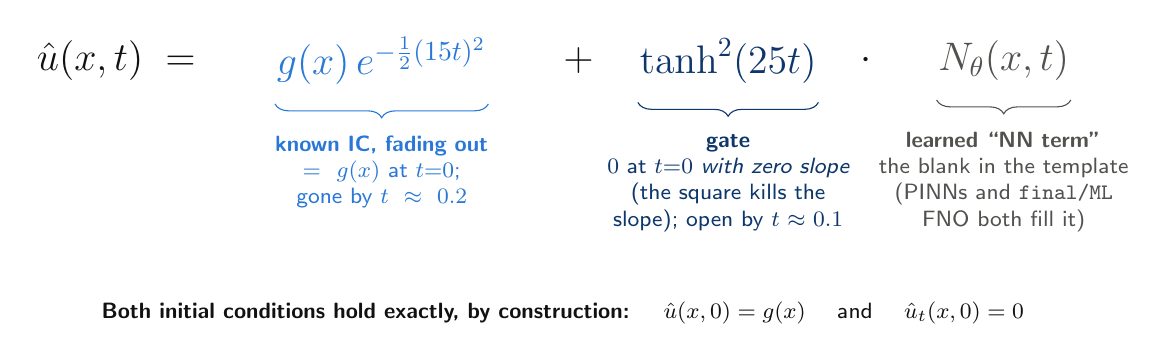
\begin{tikzpicture}
  % formula pieces as nodes on one baseline
  \node[text=ink]              (u)    at (0,0)     {\Large $\hat u(x,t) \;=\;$};
  \node[text=accent]           (ict)  at (3.3,0)   {\Large $g(x)\, e^{-\frac{1}{2}(15t)^2}$};
  \node[text=ink]              (plus) at (5.8,0)   {\Large $+$};
  \node[text=dblue]            (gate) at (7.7,0)   {\Large $\tanh^2(25t)$};
  \node[text=ink]              (dot)  at (9.45,0)  {\Large $\cdot$};
  \node[text=gray52]           (nn)   at (11.2,0)  {\Large $N_\theta(x,t)$};

  % braces + labels
  \draw[decorate,decoration={brace,mirror,amplitude=5pt},accent]
    ($(ict.south west)+(0.1,-0.12)$) -- ($(ict.south east)+(-0.1,-0.12)$)
    node[midway, below=8pt, lbl, text=accent, text width=3.7cm]
    {\textbf{known IC, fading out}\\ $=g(x)$ at $t{=}0$;\\ gone by $t\approx0.2$};

  \draw[decorate,decoration={brace,mirror,amplitude=5pt},dblue]
    ($(gate.south west)+(0.1,-0.12)$) -- ($(gate.south east)+(-0.1,-0.12)$)
    node[midway, below=8pt, lbl, text=dblue, text width=3.1cm]
    {\textbf{gate}\\ $0$ at $t{=}0$ \emph{with zero slope} (the square kills the slope); open by $t\approx0.1$};

  \draw[decorate,decoration={brace,mirror,amplitude=5pt},gray52]
    ($(nn.south west)+(0.1,-0.12)$) -- ($(nn.south east)+(-0.1,-0.12)$)
    node[midway, below=8pt, lbl, text width=3.4cm]
    {\textbf{learned ``NN term''}\\ the blank in the template (PINNs and \texttt{final/ML} FNO both fill it)};

  \node[lbl, text=ink] at (5.6,-3.2)
    {\textbf{Both initial conditions hold exactly, by construction:} \quad
     $\hat u(x,0)=g(x)$ \quad and \quad $\hat u_t(x,0)=0$};
\end{tikzpicture}
\end{document}
